\subsection{Connectivity}

\begin{frame}{Connectivity}
    \begin{enumerate}
        \item Keep track of visited vertices
        \item Select any unvisited vertex
        \item Start Breadth First Search from this vertex
        \uncover<4-7>{\item If there are still unvisited vertices, there is another component}
    \end{enumerate}
    
    \centering
    \tikzstyle{vertex}=[circle, draw, minimum size=15pt]
    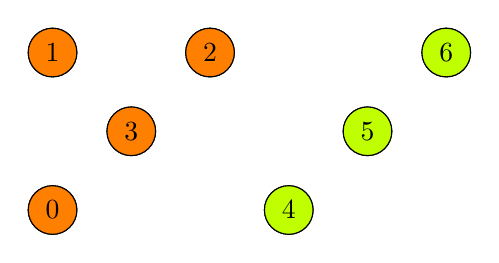
\begin{tikzpicture}[auto]
        \node<1>[vertex](0) at (0,0){0};
        \node<2->[vertex, fill=orange](0) at (0,0){0};
        \node<-2>[vertex](1) at (0,2){1}; 
        \node<3->[vertex, fill=orange](1) at (0,2){1};
        \node<-3>[vertex](2) at (2,2){2};
        \node<4->[vertex, fill=orange](2) at (2,2){2};
        \node<-2>[vertex](3) at (1,1){3};
        \node<3->[vertex, fill=orange](3) at (1,1){3};
        
        \node<-4>[vertex](4) at (3,0){4}; 
        \node<-5>[vertex](5) at (4,1){5};
        \node<-6>[vertex](6) at (5,2){6};
        \node<5->[vertex, fill = lime](4) at (3,0){4}; 
        \node<6->[vertex, fill = lime](5) at (4,1){5};
        \node<7->[vertex, fill = lime](6) at (5,2){6};
        
        \Edge (0)(1);
        \Edge (0)(3);
        \Edge (3)(1);
        \Edge (3)(2);
        \Edge (4)(5);
        \Edge (5)(6);
    \end{tikzpicture}
        
    \centering
    \uncover<2->{%
        Visited = [\only<2->{0}\only<3->{, 1, 3}\only<4->{, 2}\only<5->{, 4}\only<6->{, 5}\only<7->{, 6}]
        
        Number of components = \only<1-4>{1}\only<5->{2}
    }
\end{frame}